\begin{figure}[ht]
\tikzset{black/.style={shape=circle,draw=black,fill=black,inner sep=1pt, minimum size=9pt}}
\tikzset{white/.style={shape=circle,draw=black,fill=white,inner sep=1pt, minimum size=9pt}}

\tikzset{invisible/.style={shape=circle,draw=black,fill=black,inner sep=0pt, minimum size=0.1pt}}
\begin{center}
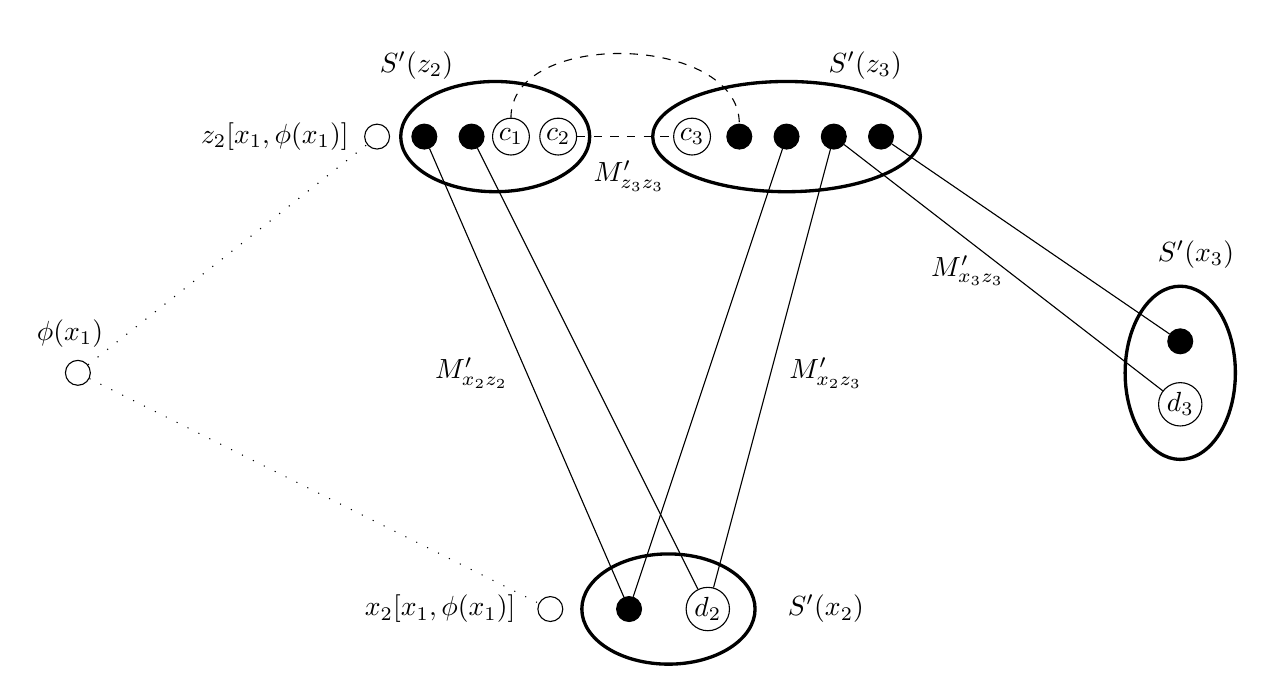
\begin{tikzpicture}
\filldraw[color=black!100, fill=black!0, very thick] (0.5,-3) ellipse (1.1 and 0.7);
\filldraw[color=black!100, fill=black!0, very thick] (7,0) ellipse (0.7 and 1.1);
%\filldraw[color=black!100, fill=black!0, very thick] (-7,0) ellipse (0.7 and 1.7);
\filldraw[color=black!100, fill=black!0, very thick] (-1.7,3) ellipse (1.2 and 0.7);
\filldraw[color=black!100, fill=black!0, very thick] (2,3) ellipse (1.7 and 0.7);

        %\node[] at (-8,0) {$x_1$};
        \node[] at (2.5,-3) {$S'(x_2)$};
        \node[] at (-2.7,3.9) {$S'(z_2)$};
        \node[] at (3,3.9) {$S'(z_3)$};
        \node[] at (7.2,1.5) {$S'(x_3)$};


        \node[white] (1) at (-7,0){};
        \node[white] (2) at (-3.2,3){};
        \node[black] (3) at (-2.6,3){};
        \node[black] (4) at (-2,3){};
        \node[white] (5) at (-1.5,3){$c_1$};
        \node[white] (6) at (-0.9,3){$c_2$};
        \node[white] (7) at (0.8,3){$c_3$};
        \node[black] (8) at (1.4,3){};
        \node[black] (9) at (2,3){};
        \node[black] (10) at (2.6,3){};
        \node[black] (11) at (3.2,3){};
        \node[black] (12) at (7,0.4){};
        \node[white] (13) at (7,-0.4){$d_3$};
        \node[white] (14) at (1,-3){$d_2$};
        \node[black] (15) at (0,-3){};
        \node[white] (16) at (-1,-3){};

        \node[] (17) at (-7.1,0.5){$\phi(x_1)$};
        \node[] at (-4.5,3) {$z_2[x_1, \phi(x_1)]$};
        \node[] at (-2.4,-3) {$x_2[x_1, \phi(x_1)]$};
        \node[] at (-2,0) {$M'_{x_2z_2}$};
        \node[] at (2.5,0) {$M'_{x_2z_3}$};
        \node[] at (4.3,1.3) {$M'_{x_3z_3}$};
        \node[] at (0,2.5) {$M'_{z_3z_3}$};



        \draw[loosely dotted] (1)--(2); 
        \draw[loosely dotted] (1)--(16); 
        \draw[black] (15)--(3); 
        \draw[black] (14)--(4); 
        \draw[black] (12)--(11); 
        \draw[black] (13)--(10); 
        \draw[black] (14)--(10); 
        \draw[black] (15)--(9); 
        \draw[out=90,in=90,dashed]  (5) to  (8);
        \draw[dashed] (6)--(7); 
        %\draw[black] (4)--(5); 
        %\draw[dashed] (2)--(13);
        %\draw[dashed] (1)--(14);

\end{tikzpicture}


\caption{The matchings between $S'(x_2)$, $S'(x_3)$, $S'(z_2)$, and $S'(z_3)$, as described in the proof of the second statement in Claim \ref{keyclaim}. The matching $M'_{x_2x_3}$ is omitted for clarity. We assume there exists a colour $d_2 \in S'(x_2)$ and $d_3 \in S'(x_3)$ such that $z_2[x_2,d_2] = z_2[x_3,d_3]$. Without loss of generality, we may assume that the solid edges in the matchings are as shown. No matter the matching $M'_{z_2z_3}$, there exist colours $c_i \in S'(z_2)$ and $c_3 \in S'(z_2)$ such that $c_i$ is unmatched in $M'_{x_2z_2}$, such that $c_3$ is unmatched in $M'_{x_2z_3}$ and $M'_{x_3z_3}$, and such that $c_3 \neq z_3[z_2, c_i]$.} 
    \label{fig:matchings2}
\end{center}
\end{figure}






